\documentclass{article}
\usepackage[utf8]{inputenc}
\usepackage{graphicx}
\usepackage{float}
\usepackage{longtable}

\title{Design Document: bike4share}
\author{Maffioli Sara, Papale Lorenzo, \\ Stucchi Lorenzo \& Vaghi Federica}


\begin{document}
\maketitle
\tableofcontents

\newpage

\section{Introduction}

The aim of the project is to develop a web application called “bike4share” for a bike sharing service in order to guarantee to the user a web service to search for the availability of bikes and free stalls around his position or the desired location in the city.\\The web application must ensure the technician to have a private section showing analytic graphs and statistics on the bike flow in real time.
The main used technologies are shown in Table 1
\begin{table} [H]
    \begin{center}
        \begin{tabular}{|l|p{0.75\textwidth}|}
            \hline
            PostgresSql & Used in order to to manage the databases        \\
            \hline
            Python & Perform the outputs, build the map and  manage the map's background 
             \\
            \hline
            Flask &  Set for the visualisation of the statistics
              \\
            \hline
        \end{tabular}
    \end{center}
\caption{Technologies overview }
\end{table}

\subsection{Purpose}
This document is a generic Technical Design Document for “ bike4share”. The purpose of this document is to outline the technical design of the web application system and provide an overview for the used databases and software.\\
It is mainly  intended to assist the customer that has invested in sustainable mobility (Municipality of Milan) and the technicians who have to monitor the system in order to work on data and extract the needed information.
\subsection{Scope}
The final output of the “ bike4share” project will be a client–server computer program which the client, including the user interface and client-side logic, runs in a web browser.
The system will allow  the user to interact with a web page in which different functions are offered to different type of users (Table 2).
The basic functions allow the not registered users to perform some elementary activities.  
The premium functions are in addiction of the basic function and they are  accessible for the users after the registration, once the log-in phase is successfully completed, the registered user can access to different functionalities that can help the usability of the app.
A specific section of the application is devoted to the technician’s use. 
The technicians are requested to complete the registration and log-in to have access to their specific section. Here it's possible, in addition to all the other functionalities, to perform some analysis and graphical statistics with specific tools.
\begin{table} [H]
    \begin{center}
        \begin{tabular}{|l|p{0.6\textwidth}|}
            \hline
            BASIC FUNCTION &   \begin{itemize}
                               \item Showing the position of all the bike stalls
                               \item ID Number of bikes stalls per each selected station
                               \item Number of the stalls for each selected station
                               \end{itemize}
        \\
            \hline
            PREMIUM FUNCTION &  \begin{itemize}
                                \item Display the position of the user on the map
                                \item Help the users to visualise the nearest station with respect to their position
                                \item Showing the list of all the available  stations nearby
                                \item Manually typing of the address or select the position on the map  
                                \end{itemize}
             \\
            \hline
            TECHNICIAN AREA &  \begin{itemize}
                               \item Plotting of the stations median bikes availability per day of the week
                               \item Plotting of the stations median bikes availability per day of the month
                               \item Plotting of the percentage of bikes availability per day
                               \item Plotting of the percentage of bikes availability per month
                               \item Bike availability trend per weekend
                               \item Real-time data previous week
                               \item Real-time data previous month
                               \item Move over the map
                               \end{itemize}
                \\
            \hline
        \end{tabular}
    \end{center}
\caption{"bike4share" functionalities overview}
\end{table}
The main advantages of “bike4share” is the possibility of planning the usage of a bicycle for the daily mobility in a sustainable way, in order to avoid delay, stress and unexpected events while there are important delivery or scheduled appointment.
The main goal is to provide to the customers, users and technician the best services as possible in terms of system performance and functionalities in order to help them with their daily objectives.
Thanks to the premium functionalities it’s possible to avoid different organisational problems. 
Even if the users don’t allow to access to the position because of privacy reasons it’s however possible to use the “bike4share” web application thanks to the manual typing of the addresses.  
The log-in, e-mail address and password request are able to reduce the security risks for the users and the main risk related to the usage of this application in case of a security hack will be related to the acquisition of data regarding the positions of the users.
\subsection{Definitions, acronyms and abbreviations}
DB:database\\
DBMS: database management system\\
b4s: bike4share\\
HW: hardware\\
SW: software\\
DD: Design Document
\subsection{Document Organization}
This document is organized in different sections like described in Table 3.

\begin{table} [H]
    \begin{center}
        \begin{tabular}{|l|p{0.6\textwidth}|}
            \hline
            Introduction &   Provides information related to this document         \\ 
            \hline
            Design Overview &  
            Describes the approach, architectural goals and constraints \\
            \hline
            System Architecture &  
            Describes s the various system components and their integration \\
            \hline
            Data Design & Outlines the design of the DBMS and non-DBMS files \\
            \hline
            Detailed Design & Describes the proposed design in detail 
            \\
            \hline
             Human-Machine Interface & Describes the proposed interface
            \\
            \hline
        \end{tabular}
    \end{center}
\caption{Document organization}
\end{table}
\newpage
\section{Design Overview}
This section briefly introduce the system context and design, and discuss the background to the project
\subsection{Approach}
The “bike4share” Web Application is created and extended in multiple phases over the course of the project (Table 4).
\begin{table} [H]
    \begin{center}
        \begin{tabular}{|l|p{0.6\textwidth}|}
            \hline
            Requirements Phase &   Describing the candidate architecture to be validated         \\
            \hline
            System Design Phase &  
            Describes the approach, architectural goals and constraints \\
            \hline
            Prototype Phase &  
            Evolutionary Prototype and the architectural foundation is created    \\
            \hline
            Construction Phase & Technical procedure for the tasks is defined \\
            \hline
            Training Phase & Test of the final product
            \\
            \hline
        \end{tabular}
    \end{center}
\caption{Phases of the project's developement}
\end{table}

\subsection{Background Information}

The  customer has invested in sustainable mobility by installing a number of bike stalling stations around the City. The implemented bike sharing system must be monitored with the “bike4share” WebApp for assessing the bikes flow both in space and time and, eventually, for designing future system improvement actions. 
Also, the customer has the need to inform in real time bike sharing users about the status of each stations.

\subsection{Constraints}
\begin{longtable}{|p{0.22\textwidth}|p{0.75\textwidth}|}
    
    \hline
    TECHNICAL CONSTRAINTS &         \begin{itemize}
                                    \item PostgreSQL
                                    \item Python-Flask 
                                    \item Python-Bokeh
                                    \item Python data analysis and plotting
                                    \item A vector map of the stalling stations (shapefile)
                                    \end{itemize}
                \\
    \hline
      DELIVERY CONSTRAINTS &        \begin{itemize}
                                    \item First version of requirement analysis document on the 29th of April in 2019.	
                                    \item First version of the Design Document and Test Plan are scheduled on the 26th of May in 2019.
                                    \item Implementation, test report and updated document scheduled on the 09th of June in 2019. 
                                    \end{itemize}
             \\
            \hline
\caption{Constraints overview} \\
\end{longtable}

\subsection{ Design Trade-offs}
The trade-off method used in the development of the “bike4share” application is based on the functional and quality requirements of the predicted system, a number of scenarios was created in order to  represent both the day-to-day use, and the intended use of the Premium  Functionality introduced (ref cap 2.8.1). 
Using these scenarios, different functional parts are then extracted from architecture descriptions prepared for each of the use-case scenarios. Since the evaluation is conducted at the architecture level, the different parts can cover measures such as the number of active data repositories, passive data repositories, persistent and non-persistent components, data links, control links, logical groupings, styles and patterns and violations of the intended architecture. These metrics are collected by the developer of the whole system that estimate complexity, impact and effort for each of the scenarios for each of the architectures using an existing architecture as a point of reference (for example the BikeMi services). Based on the collected metrics it is then possible to compare the architecture alternatives and based on that select the most appropriate architecture for the improvement of the system. The alternative architectures are assessed with mainly respect to robustness but they are also compared for reliability, maintainability, interoperability, portability, scalability and performance.

\subsection{User Characteristics}
There are different kind of users. Every user can interact with different information about the bike stalls placed in Milan (Table 6). 

\begin{table} [H]
    \begin{center}
        \begin{tabular}{|p{0.22\textwidth}|p{0.75\textwidth}|}
            \hline
            REGISTERED USER &   A user that is registered yet and that wants to access the “b4s” web application services in order to use the premium functions available  on  the application. It  could  be  a  person  that  uses this service frequently. \\ 
            \hline
            NOT REGISTERED USER &  
            A user  that  isn’t registered  yet  and  that  wants to ccess  the  “b4s”  web application  services  in  order  to  use the  basic functions available on the application, it could be a person that doesn’t use this service frequently or a new user that wants to start an approach to this service and try it for the first time  \\
            \hline
            TECHNICIAN &  
            A person who is authenticated thanks to specific credential given by the master of the service and who has been granted supervising permissions.   He/she  is  allowed  to  view,  analyze,  access  statistics  and aggregated information about the “b4s” web application services.
            \\
            \hline
        \end{tabular}
    \end{center}
\caption{User-type description}
\end{table}

\subsubsection{User Problem Statement}
In this section the main problems that a user could have by experiencing the “b4s” web application are described.
It is possible to identify the following problems with respect to the type of event that is occurring .

\begin{longtable}{|l|p{0.6\textwidth}|}
    \hline
    USER'S PROBLEM      &         TYPE OF EVENT    
      \\
    \hline
      
      REGISTRATION PHASE  &        \begin{itemize}
                                   \item User name already existed: the username already exists and it is proposed to change the chosen username
                                   \item  E-mail already existed: the e-mail already exists, so an error is shown and it is proposed to change the chosen e-mail
                                   \item  Incorrect e-mail address: the format of the mail is wrong so the system requires to correct it and to insert a valid one
                                   
                                   \item Invalid secret-key(only technician's problem):it can be solved by contacting the administrator
                                   \end{itemize} 
                \\
    \hline
      LOG-IN PHASE &        \begin{itemize}
                            \item Forgot password:the user can follow the recovery password procedure
                            \item Localization doesn’t work: so the system provides to the logged user the possibility of  manually inserting the needed address and find the position or adding a point in his position
                            \item Maps providers crash
                            \item Server doesn’t work
                            \end{itemize}
             \\
            \hline
\caption{User's problem overview} \\

\end{longtable}

\section{System Architecture}
Our web application “bike4share” will work thanks to several components supporting it.
We can recognise three levels of the system: User, Software and Data, as is showed in figure \ref{fig:schema}. 
\begin{figure}[H]
    \centering
    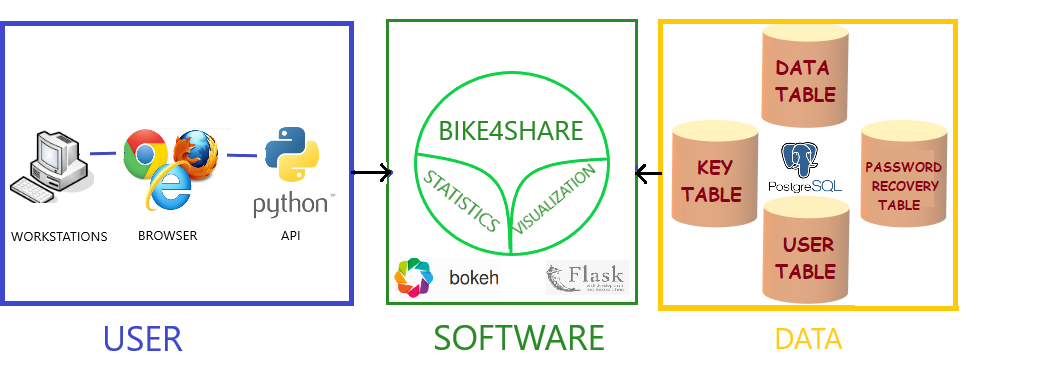
\includegraphics[width=0.75\linewidth]{image/BIKE4SHARE_SCHEMA_FINAL.png}
    \caption{Overall view of "bike4share" system architecture}
    \label{fig:schema}
\end{figure}
Starting from the right and considering the inputs, Data are retrieved from four Databases, one for the registered users and technicians, one for the information regarding the data of the bike stations, one for the password recovery procedure and one for the secret key created for the first log-in of the technician.
The outputs of “b4s”, instead, are the visualisation of a map showing the bike stations with the relative information (bikes and free stalls) and the visualisation of statistics (only for technicians)and they are showed in the middle of the Figure 1. On the left there is the section regarding to the user, capable of viewing the map to obtain the information, and the technician, who can analyse data and statistics. Both the actors can perform their purposes accessing the page through the browser.
\subsection{Hardware Architecture}
As seen in the previous paragraph, the Bike4share is designed as a distributed system: a three-layers architecture. A graphical description is shown in the figure \ref{fig:over}.
\begin{figure}[h]
    \centering
    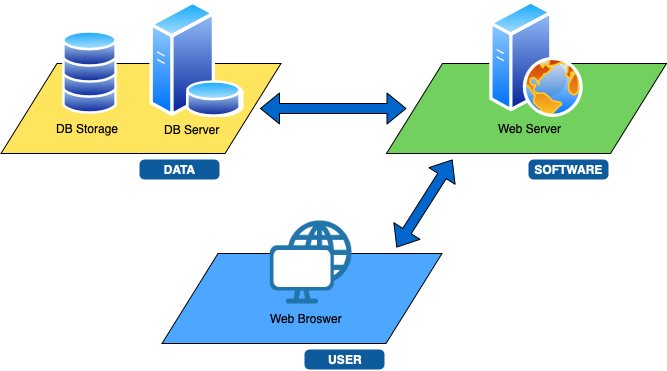
\includegraphics[width=0.55\linewidth]{image/hardware_COMPLETE.png}
    \caption{Overall view of "bike4share" hardware architecture}
    \label{fig:over}
\end{figure}

\begin{itemize}
    \item Database Server: This component, which includes also the DB storage, provides all the data when requested by the application (with SQL queries), allowing it to accomplish its functionalities.
    \item Web Server: It is focused on the workflow and it is responsible for the communication with both the Database Server and the User.
    \item Web Browser: The role of this component is crucial for what concerns the interface, the user information retrieval (for registration and login) and the presentation of the information needed by the User and by the Technician. 
\end{itemize}
It is important to consider the fact that in the programming phase the architecture of the system is centralised. Since the system involves the use of a single machine, the role of all the components is played by the machine itself as shown in the figure \ref{fig:com_createSchema}.\\
\begin{figure}[H]
    \centering
    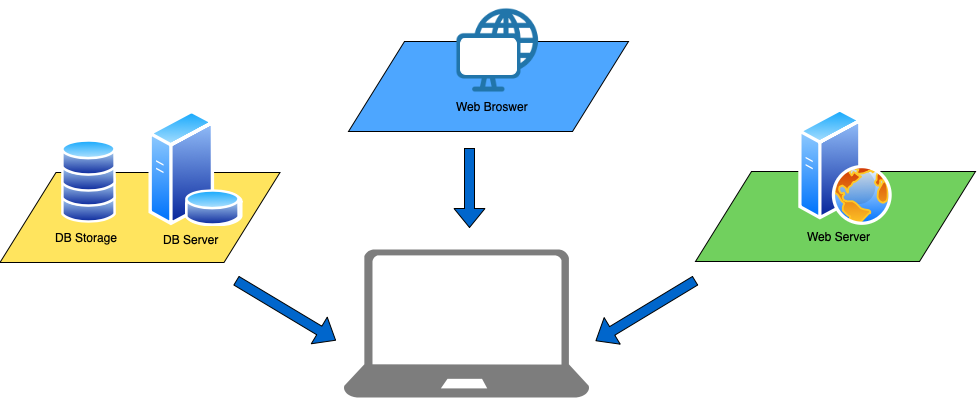
\includegraphics[width=0.85\linewidth]{image/hardware_architecture.png}
    \caption{"bike4share" hardware architecture during system creation phase}
    \label{fig:com_createSchema}
\end{figure}

\subsection{Software Architecture}
The software architecture is mainly based on the implementation of the statistics thanks to Bokeh and the visualization of the obtained results through flask.
The programming language is Python and in particular the libraries and the tools that are used are:

\begin{longtable}[H]{|p{0.2\textwidth}|c|p{0.6\textwidth}|}
    \hline
    Packages Name & Version & Description \\    
    \hline
      Pandas  & 0.24.2    &   It provides high-performance, easy-to-use data structures and data analysis tools for the Python programming language
                \\
    \hline
      Geopandas & 0.4.1 &     It combines the capabilities of pandas and shapely, providing geospatial operations in pandas and a high-level interface to multiple geometries to shapely random function 
             \\
    \hline 
    Psycopg2 & 2.8.1 & The most popular PostgreSQL DB adapter for the Python programming language. It was designed for heavily multi-threaded applications. It features client-side and server-side cursors, asynchronous communication and notifications, many Python types are supported out-of-the-box and adapted to matching  PostgreSQL data types; adaptation can be extended and customized thanks to a flexible objects adaptation system
               \\
    \hline
    Sqlalchemy & 1.3.2 & It is the Python SQL toolkit and Object Relational Mapper that gives application developers the full power and flexibility of SQL. It provides a full suite of well known enterprise-level persistence patterns, designed for efficient and high-performing database access, adapted into a simple and Pythonic domain language
       \\
    \hline
    Geoalchemy2 & 0.6.1 & It provides extensions to SQLAlchemy for working with spatial DBs and it is focused on PostGIS
      \\
    \hline
    GeoJSON & 2.4.1 & Is a format for encoding a variety of geographic data structures that supports the following geometry types: Point, LineString, Polygon, MultiPoint, MultiLineString, and MultiPolygon. Geometric objects with additional properties are Feature objects. Sets of features are contained by FeatureCollection objects
       \\
    \hline
    Bokeh & 1.1.0 &  It is an interactive visualization library its goal is to provide elegant, concise construction of versatile graphics, and to extend this capability with high-performance interactivity over very large or streaming datasets
        \\
    \hline
    Flask & 1.0.2 & It is a micro web framework written in Python that supports extensions that can add application features as if they were implemented in Flask itself. Extensions exist for object-relational mappers, form validation, upload handling, various open authentication technologies and several common framework related tools \\
    \hline
    Werkzeug & 0.14.1 & Werkzeug is a comprehensive WSGI web application library
    \\
    \hline
    psycopg2 & 2.8.1 & psycopg is the most popular PostgreSQL adapter for the Python programming language. At its core it fully implements the Python DB API 2.0 specifications
    \\
    \hline
    PgAdmin & 4.5 & It is a management tool for PostgreSQL and derivative relational databases such as EnterpriseDB's EDB Advanced Server
        \\
    \hline
    Leaflet & 1.4.0 & It is the leading open-source JavaScript library for mobile-friendly interactive maps, it has all the mapping features most developers need.It works efficiently across all major desktop and mobile platforms, can be extended with lots of plugins and it is an easy to use  API 
       \\
    \hline
    Leaflet-knn & 0.1.0 & In order to compute the distance between the points and returning the nearest one it is used the external functions called leaflet-knn with the relative license (https://github.com/mapbox/leaflet-knn)
    \\
    \hline
    Leaflet Control Geocoder & 1.8.2 & This package allows to insert manually an address returning the position on the map\\
    \hline
\caption{Software architecture packages and tools}
\end{longtable}

The structure of the software is based on the following python script and reusable functions as it is shown in the table 9.
\newpage

    \begin{longtable}[H]{|l|p{0.7\textwidth}|} 
  
    \hline
    NAME      &         DESCRIPTION AND FUNCTIONS
      \\
      \hline
    createSchema.py &  It allows the creation of the different table used by the  “bike4share” WebApp. Thanks to the SQL query and the pgAdmin DBs connection it is possible to access, create, updated, extract data and fill the different DBs which interact with the user side in order to guarantee the consistency with the latest version of the data
      \\
    \hline 
    realtime\_data.py & It allows the data analysis in real-time thanks to the connection with the DBs
    \\
    
    \hline
    func.py & It is a function that allow to send an email to the user in order to send back an e-mail containing the recovery code for the forgot password procedure. it'll take the e-mail address and the random code of the users automatically from the DBs. for the generation of the code the following function is used:
      \begin{itemize}
         \item Key\_generator: it is a function defined in order to automatically generate some random password that will be given to the technician directly from their chief or by our customer (the buyer of the system, the Municipality of Milan)
    \end{itemize}
    \\
    \hline 
   Statistics.py & It is the section of “bike4share”software development that  allows to creation of plots, representing the different evaluated statistics. The principal functions are:
     \begin{itemize}
          \item pd.to\_datetime: Pandas function to convert string date time into Python date time object
          \item df\_bike.groupby: it allows to split the data into groups based on some criteria
          \item ColumnDataSource: it allows to store the data to use in the bokeh graph
          \item figure: it allows to create a new figure in Bokeh
          \item callback: it allows to upload the graph
          \item getPointCoords: it allows to retrieve coordinates from the geodataframe 
     \end{itemize}
       \\
    \hline
    main.py & It is the main part of “bike4share”software development, it allows to log-in, access,register, make some statistics and visualise the map in which the bike and stalls information thanks to the direct connection to the DBs with the following main function:
     \begin{itemize}
     
         \item get\_dbConn: it allows the connection with the  DBs
         \item close\_dbConn: it allows the disconnection from the  DBs
         \item load\_logged\_in\_user: it allows to check if the user is inserted yet in the user’s DB and make the consequent operations
         \item index: it allows the map visualization
         \item register: it allows the registration of the user
         \item log\_in: it allows the log-in of the pre-registered users
         \item forgotpassword: it allows to recovery the forgotten password both for the users than the technician
         \item set\_new\_password: it allows both the user and the technician to set a new password and store it in the DB instead of the old forgotten one
         \item log\_out: it allows the log-out of the users 
         \item tech\_reg: it allows the registration of the technician
         \item bash\_command: it allows the bokeh application running on port 5006 to be accessed at port 5000 by Flask
         \item statistics: it allows Flash to read what is the bokeh server and to have access to the statistics.
     \end{itemize}
     \\
    \hline
    downloadStation.py & It allows to download the data about the station from the DB and to save it to a GeoJSON file and trasform it into a javascript variable. 
      \\
    \hline
\caption{Software structure overview } \\
\end{longtable}
      
\subsection{Communications Architecture}
The Communication diagram, fig \ref{fig:createSchema}, is a diagram that shows the interactions between elements at run-time. They  are used to visualize inter-object relationships.
In the schema in fig. \ref{fig:createSchema} is possible to notice how the createSchema python code is linked with the DB and how it can interact in the creation, modification and update of the dataframes.

\begin{figure}[H]
    \centering
    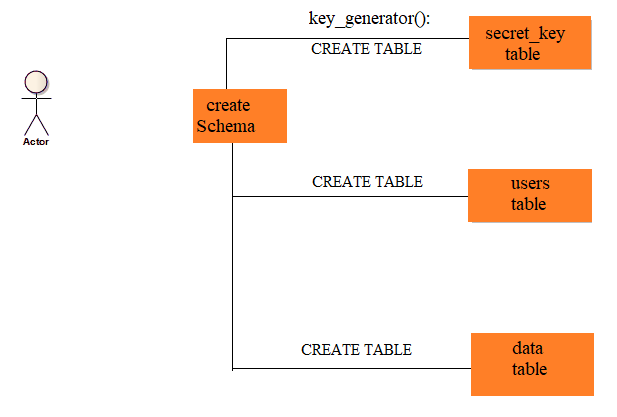
\includegraphics[width=0.65\linewidth]{image/COMM_TAB.png}
    \caption{Communication diagram related to the createSchema module}
    \label{fig:createSchema}
\end{figure}
In the figure \ref{fig:webpage} is possible to see how the different modules of the “bike4share” application are linked, what kind of function are used and how they interact between themselves.

\begin{figure}[H]
    \centering
    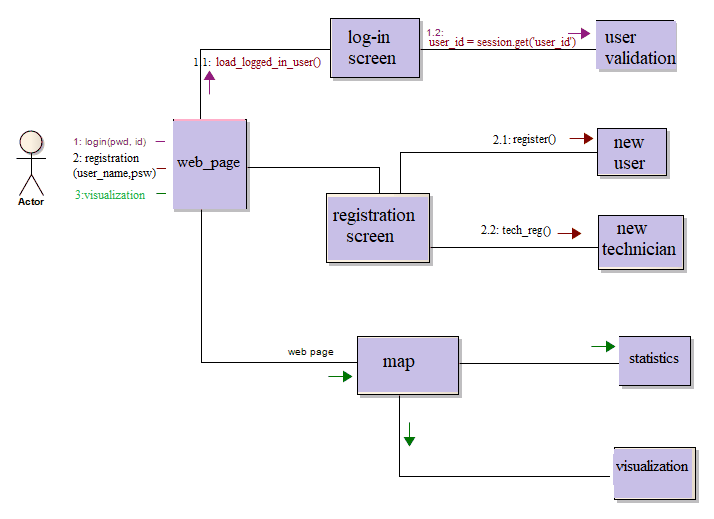
\includegraphics[width=0.75\linewidth]{image/comunication_architecture.png}
    \caption{Communication diagram related to the webpage module}
    \label{fig:webpage}
\end{figure}


\section{Data Design}
The DBMS chosen for this purpose is PgAdmin4 and the DB is mainly composed by different tables:
\begin{table} [H]
    \begin{center}
        \begin{tabular}{|l|p{0.6\textwidth}|}
            \hline
            Key\_list &  This table contains the random generated passwords for the first registration of the technician,once that one of those password is been used it’ll be deleted. \\ 
            \hline
            User\_bike  & This table contains the credentials of all the registered users in order to allow them to perform the log-in procedure. It’s checked, filled and updated every time that a new user try to make the registration  
            \\
            \hline
            Stations & This table contains the all the data related to the stations information, e.g. the address, the stalls...
            \\
            \hline
            password\_recovery & This table contains all the needed information in order to perform the forgot password procedure
            \\
            \hline
        \end{tabular}
    \end{center}
\caption{DBMS tables components}
\end{table}
\newpage
\subsection{Database Management System Files}
In this section will be described how the DB will be designed. 
In the fig \ref{fig:flow} is shown the suggested mental approach to the "b4s" application and the relationship with the corresponding DB tables. The users can navigate starting from the web application and have to think about the different choices to do in relationship with their purposes. 

\begin{figure}[H]
    \centering
    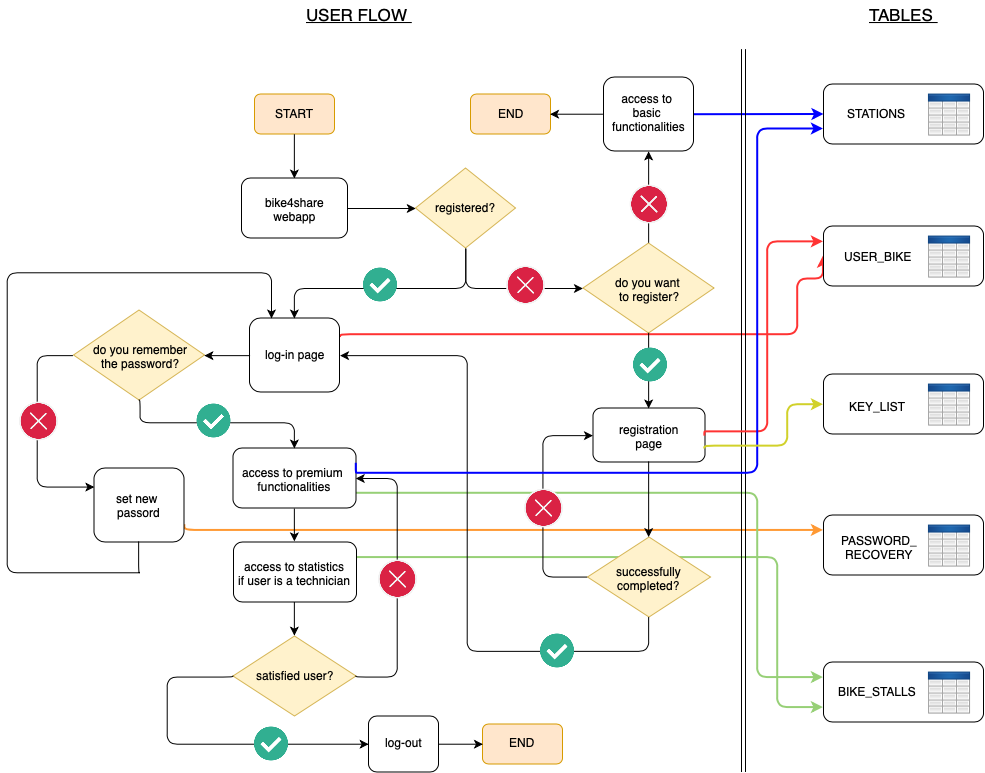
\includegraphics[width=0.99\linewidth]{image/flowchart.png}
    \caption{Representation of the flow of the events related to the usage of the b4s}
    \label{fig:flow}
\end{figure}

The table 11 will show the main attributes that describe the DB tables.
\\ 
\begin{longtable}{|p{0.18\textwidth}|p{0.18\textwidth}|l|p{0.12\textwidth}|p{0.12\textwidth}|}
 \hline TABLE NAME &   TABLE COMMENTS &    COLUMN NAME & DATA TYPE & DATA LENGTH    \\
 \hline
 KEY\_LIST &  Random  & Id\_key &int(PK)& - \\ 
 & technician passwords &  secret\_key & varchar & 35 \\
 \hline
 STATIONS  &   Informations   & ID &int & - \\
  & regarding & BIKE\_SH & text & - \\
  & stations & INDIRIZZO & text & - \\
  & & STALLI & int & - \\
  & & LOCALIZ & text & - \\
  & & LATITUDINE & double & - \\
  & & LONGITUDINE & double & - \\
 \hline
 USER\_BIKE &  Informations & user\_id & int(PK)& -\\
 & regarding & user\_name & varchar & 255 \\
 & users & user\_password & varchar & 255 \\
 & & user\_type & varchar & 255\\
 \hline 
 PASSWORD\_ &  Informations  & id\_psw & int(PK)& -\\
 RECOVERY & regarding & psw\_recovery & varchar & 11 \\
 & users who have forgotten their password & user\_name & varchar & 255 \\
 \hline
\caption{Database structure} \\
\end{longtable}

\section{Detailed Design}
\subsection{Software Detailed Design}
In this section the different module composing the “bike4share” web application will be described and commented.

\subsubsection{Module 1: CreateSchema}
In this module it is possible to create the different table stored in the DB.
\paragraph{CreateSchema: Processing}
The first operation that is made in this module is the dropping of the existing table in order to avoid inconsistency of data. After that it’s possible to create the tables (key\_list, user\_bike and password\_recovery) with all the needed parameters.
The key\_list table is filled thanks to the function key\_generator() that is able to generate different random password composed by chars, numbers and special characters value for a defined number of time; in this way is possible to check the quantity of allowed technician and to check if their password are used yet.
Also the table stations, with the information about the position of the stalls is created into the database. After the availability for every station is added in to table bike\_stalls. 

\paragraph{Local data structures}
The main structures used to store data are data frames.

\subsubsection{Module 2: downloadStation}
This module is used to download the data of the stations directly from the server, it is automated and it’s imported by the main module.

\paragraph{downloadStation: Processing}
It implies the creation of a geojson file with the information about the position and the number of stalls for every station.

\subsubsection{Module 3: realtime\_data}
This module is used to download the data of the availabilty of bikes for each station directly from the server, it is automated and it’s imported by the main module.

\paragraph{realtime\_data: Processing}
It implies the creation of a geojson file with the information about the number of free stalls and bike available for every station.

\subsubsection{Module 4: Main}
This module is the main module of the “b4s” system used to create the general schema of the website in order to connect the different sections: map, login, logout, registration, forgot password, set new password and statistics.
\paragraph{main: Processing}
The first point consists in the creation of the application instance. Then different functions are implemented to establish the connection with the DB such as get\_dbConn() and close\_dbConn(). The different sections are connected through the functions shown in Table 9.All the URLs are defined as routes in the Flask application through the app.route decorator. 
\paragraph{main: Local data structures}
The main structures used to store data are data frames and lists.

\subsubsection{Module 5: statistics}
The aim of  this module is to create different statistics on the base of the data retrieved by the DB, from tables ‘bike\_stalls’ and ‘stations’.
\paragraph{statistics: Processing}
The first operation that is made in this module is the connection to the DB in order to store the tables, above mentioned, of the data respectively in two different data frames. In this way is possible to extract the information needed to compute statistics, e.g. day and month. Functionalities to retrieve real time data have been implemented too. The data can be stored in data frames using the function df\_bike. groupby on the base of the different criteria as the median and the total availability of bikes. Using Bokeh functions it is possible to plot these statistics and to design the relative widgets. 
\paragraph{statistics: Local data structures}
The main structures used to store data are data frames and lists.
\section{Human-Machine Interface}
The user interface is easy and intuitive, fig \ref{fig:usageb4s}. When the webpage is opened, a map appears on the screen. The map shows the bike stations (as markers) in terms of position in space, with the possibility to interact with it; clicking on them, the user can immediately know what is the address and the capacity (total number of stalls)
\\
\begin{figure}[H]
    \centering
    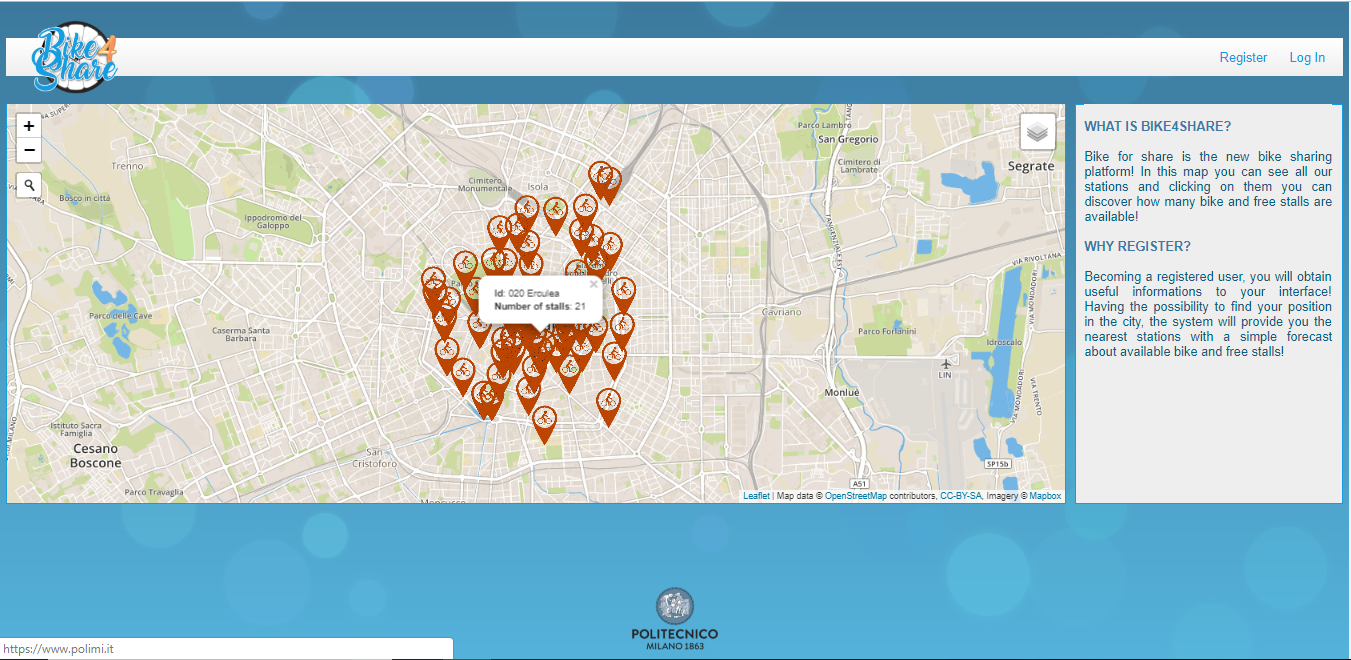
\includegraphics[width=0.8\linewidth]{image/all.PNG}
    \caption{homepage overview}
    \label{fig:usageb4s}
\end{figure}

\subsection{Interface Design Rules}
As design rule, the webpage is provided with the constant presence of the navigation bar on the top of the page.
the webpage is distinguished between the user-side and the technician-side, in the specific it contains the following buttons for the users:
\begin{itemize}
    \item Bike4share (returning the homepage)
    \item Register
    \item Log In
\end{itemize}
This design rule can help the user in navigating on the webpage with the possibility to return to the home page if something goes wrong.

\begin{figure}[H]
    \centering
    
\includegraphics[width=1\linewidth]{image/bar.PNG}
    \caption{Detail representing the navigation bar}
    \label{fig:navbar}
\end{figure}
For the technician there is also a button called "Technical Area" that allows them to access at their private session and to have access to the statistics. 

\begin{figure}[H]
    \centering
    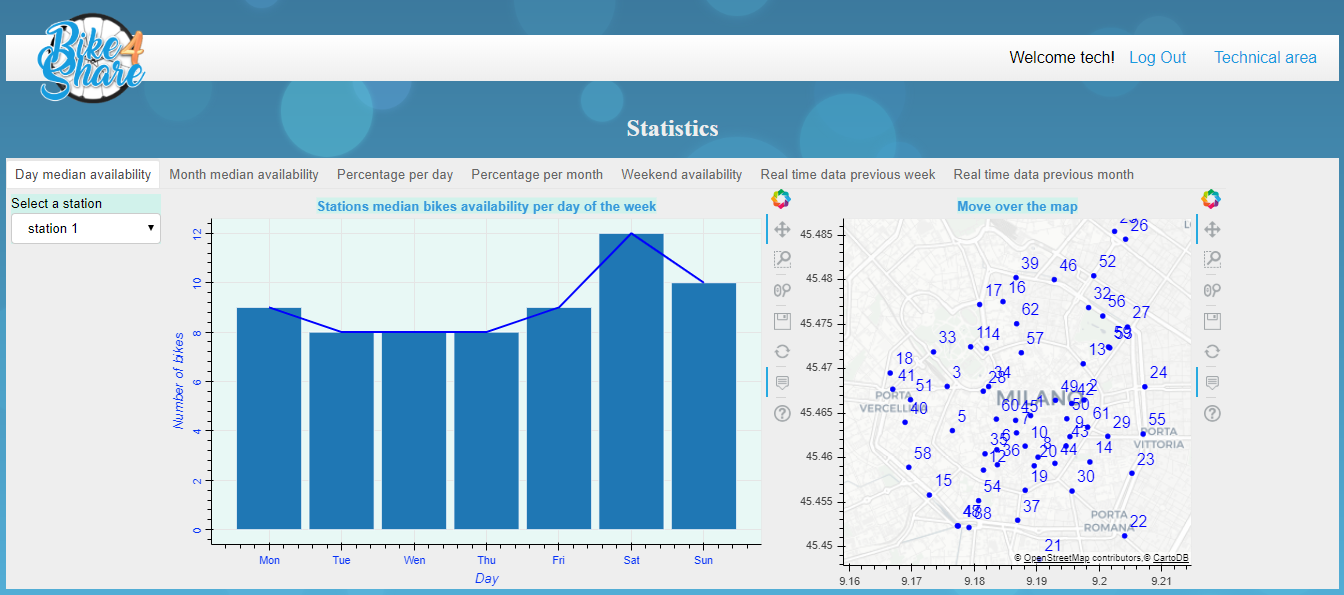
\includegraphics[width=0.8\linewidth]{image/tech.PNG}
    \caption{technical area overview}
    \label{fig:usageb4s_stat}
\end{figure}

\subsection{Inputs}
Because of the diversity of the users there will be different inputs requests. These inputs will be used in order to provide to the user the "b4s" services.

\begin{longtable}{|l|p{0.6\textwidth}|}
            \hline
            NOT REGISTERED USER &  inputs are not required; the user accesses the "b4s" web application in order to visualise the map and the relative stalls position or the total number of bikes \\ 
            \hline
            REGISTERED USER  & inputs are required for the different procedures: \begin{itemize}
                \item registration: username, password, e-mail, authorisation to GPS access 
                \item log-in: username, password
                \item forgot password: username, e-mail
                \item set new password password: username, received code, new password
            \end{itemize}
            \\
            \hline
            TECHNICIAN &  inputs are required for the different procedures: \begin{itemize}
                \item registration: username, password, e-mail, secret key, authorisation to GPS access
                \item log-in: username, password
                \item forgot password: username, e-mail
                \item set new password password: username, received code, new password
            \end{itemize}
            \\
            \hline
\caption{Input requirements} \\
\end{longtable}
        
 All these input data will be stored in the DB (the password will be hashed for security purpose) and will be checked in the DB.
 
\subsection{Outputs}
The "b4s" web application provides several outputs, based on the type of user who is logged in.

\begin{longtable}{|l|p{0.6\textwidth}|}
            \hline
            NOT REGISTERED USER &  The output provided by are:
            \begin{itemize}
            \item Map visualisation
            \item Position of the stations
            \item Total number of the stalls
            \item Name and ID of the station 
            \end{itemize}
            Map visualisation the user is allowed to know the address of each station and it's capacity. \\ 
            \hline
            REGISTERED USER  & The output provided are:
            \begin{itemize}
            \item Map visualisation
            \item Position of the stations
            \item Manual inserting of the user's position
            \item Automatic localisation
            \item List of the nearest stalls
            \item Total number of the stalls
            \item Number of free bikes available
            \item Number of free stalls available
            \item Name and ID of the station 
            \end{itemize}
            \\
            \hline
            TECHNICIAN &  The output provided are:
            \begin{itemize}
            \item Map visualisation
            \item Position of the stations
            \item Manual inserting of the user's position
            \item Automatic localization
            \item List of the nearest stalls
            \item Total number of the stalls
            \item Number of free bikes available
            \item Number of free stalls available
            \item Name and ID of the station 
            \item Statistic visualisation (Table 2)
            \end{itemize}
            \\
            \hline
\caption{input requirements} \\
\end{longtable}

\subsection{Navigation Hierarchy}
In this section is possible to find a diagram, fig \ref{fig:navigation}, of the navigation hierarchy where is shown how a user can move through the interfaces.\\
\begin{figure}[H]
    \centering
    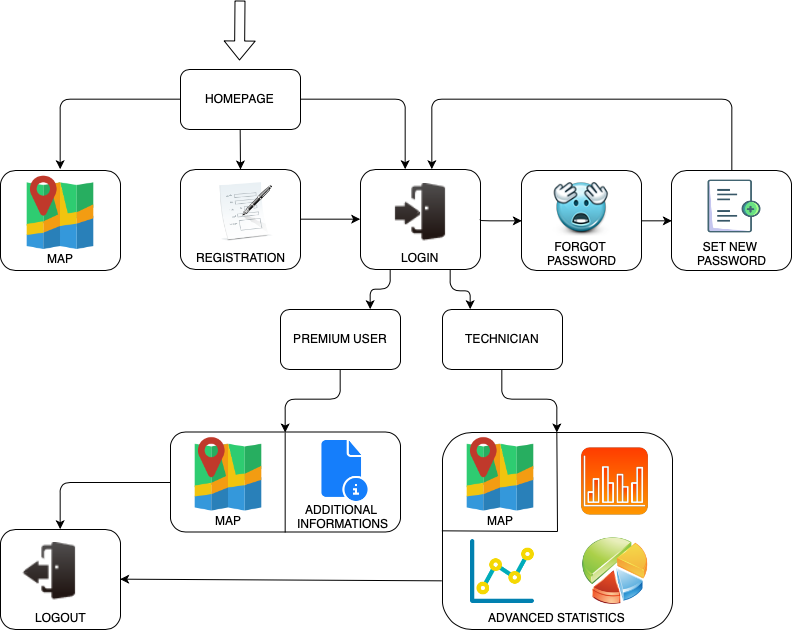
\includegraphics[width=0.68\linewidth]{image/USERFLOW2.png}
    \caption{Diagram of the navigation hierarchy}
    \label{fig:navigation}
\end{figure}

\end{document}